\documentclass{article}

% if you need to pass options to natbib, use, e.g.:
%     \PassOptionsToPackage{numbers, compress}{natbib}
% before loading neurips_2026

% ready for submission
\usepackage{neurips_2026}

% to compile a preprint version, e.g., for submission to arXiv, add the
% [preprint] option:
%     \usepackage[preprint]{neurips_2026}

% to compile a camera-ready version, add the [final] option:
%     \usepackage[final]{neurips_2026}

% to avoid loading the natbib package, add option nonatbib:
%    \usepackage[nonatbib]{neurips_2026}

\usepackage[utf8]{inputenc} % allow utf-8 input
\usepackage[T1]{fontenc}    % use 8-bit T1 fonts
\usepackage{hyperref}       % hyperlinks
\usepackage{url}            % simple URL typesetting
\usepackage{booktabs}       % professional-quality tables
\usepackage{amsfonts}       % blackboard math symbols
\usepackage{nicefrac}       % compact symbols for 1/2, etc.
\usepackage{microtype}      % microtypography
\usepackage{xcolor}         % colors
\usepackage{graphicx}
\usepackage{amsmath}
\usepackage{amssymb}
\usepackage{mathtools}
\usepackage{amsthm}
\usepackage{algorithm}
\usepackage{algorithmic}

\title{Evo-Distill: Distilling Evolutionary Search into One-Shot Policies}

\author{%
  Anonymous Author \\
  Affiliation \\
  Address \\
  \texttt{email} \\
}

\date{}

\begin{document}

\maketitle

\begin{abstract}
Evolutionary Algorithms (EA) are robust global optimizers but suffer from high sample complexity. Existing work views EA and Deep Learning (DL) as alternative solvers, or uses one to tune the other. We propose a fundamentally different perspective: \textbf{EA as a Fixed-Point Operator} that maps an initial population to a basin of attraction, and \textbf{Transformer as a Function Approximator} of this operator.

We introduce \textbf{Evo-Distill}, a framework that distills the entire evolutionary search trajectory into a causal \emph{Genealogical Graph Transformer}. Unlike standard sequence models, Evo-Distill explicitly models the ``procedural topology'' of search---identifying which mutation or crossover events led to fitness breakthroughs. By training on offline EA traces, the model learns a ``one-shot evolution'' policy: given a problem instance and a cheap initial population, it predicts the final elite solution in a single forward pass, bypassing thousands of function evaluations. We demonstrate that this amortized \emph{fixed-point learning} achieves $>10\times$ evaluation efficiency on expensive black-box optimization benchmarks compared to running the EA teacher online.
\end{abstract}

\section{Introduction}
\label{sec:intro}

Evolutionary Algorithms (EAs) are indispensable for optimizing non-differentiable, rugged, or deceptive landscapes, finding applications in fluid dynamics design, molecular discovery, and reinforcement learning. However, their reliance on population-based stochastic search incurs a massive computational cost---often requiring $10^4$--$10^6$ function evaluations to converge. When each evaluation involves a high-fidelity simulation (e.g., CFD or ab initio calculations), standard EA becomes prohibitively expensive.

Current approaches to accelerate optimization fall into two camps: (1) \emph{Meta-Learning / Learned Optimizers} (L2O), which learn gradient-based update rules; and (2) \emph{Surrogate-Assisted EA}, which approximate the fitness landscape. Both have limitations: L2O struggles with the deceptive local optima that EAs handle well \cite{metz2022learned}, while surrogates often fail to capture the global topology of the search space.

\paragraph{EA as a Fixed-Point Operator.}
We propose a third path: \textbf{Amortized Evolutionary Search}. We observe that for a given family of problem instances $p \sim \mathcal{P}$, an EA $\mathcal{E}$ acts as a deterministic operator in distribution space, mapping an initial population state $\mathcal{S}_0 = (p, \mathcal{P}_0)$ to a final converged state $\mathcal{S}_T$ containing elite solutions $x_\star$ (Figure~\ref{fig:fixed_point}). 
Crucially, the \emph{trajectory} of the EA $\tau = (\mathcal{P}_0, \dots, \mathcal{P}_T)$ contains rich structural information about the landscape's geometry---specifically, which ``genealogical paths'' of mutation and crossover succeeded where random search failed.

\begin{figure}[b]
    \centering
    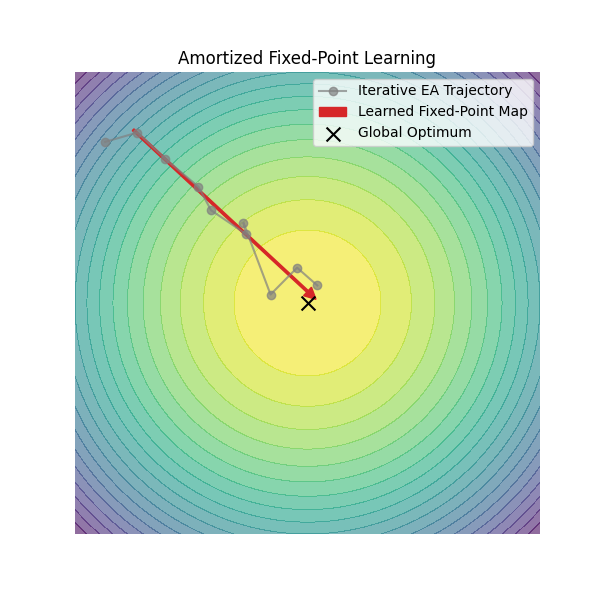
\includegraphics[width=0.8\linewidth]{figs/fixed_point.png}
    \caption{\textbf{Fixed-Point Operator Learning.} Traditional EAs (grey path) iteratively traverse the fitness landscape, slowly converging to the global optima. Evo-Distill (gold path) learns the direct ``fixed-point mapping'' from the initial population distribution to the basin of attraction, effectively amortizing the search cost into a single forward pass.}
    \label{fig:fixed_point}
\end{figure}

\paragraph{Evo-Distill.}
We venture to learn the fixed-point mapping $\Phi: (p, \mathcal{P}_0) \mapsto x_\star$ directly. We introduce \textbf{Evo-Distill}, which treats the EA trajectory not as a flat sequence, but as a \textbf{Genealogical Graph}.
\begin{enumerate}
    \item \textbf{Graph-Structured Attention}: We represent the population history as a Directed Acyclic Graph (DAG) where edges denote genealogical relationships (parent $\to$ offspring). The model uses masked attention to trace the ``lineage of success,'' learning to attend to ancestors that contributed to fitness jumps.
    \item \textbf{Contrastive Utility Learning}: Rather than imitating every step (which includes many neutral or deleterious mutations), we employ a utility-weighted loss that prioritizes learning from transitions with high positive fitness gain ($\Delta f > 0$).
    \item \textbf{One-Shot Amortization}: At inference time, Evo-Distill predicts the EA's fixed point in a single pass. This serves as a ``super-initialization'' that places the search directly in the high-fitness basin, reducing the need for costly exploration.
\end{enumerate}

At inference time on a new instance $p'$, Evo-Distill consumes the problem description, a cheaply obtained initial population (e.g., random or heuristic-based), and optionally a few initial EA steps. It then outputs a candidate elite $\hat{x}_\star^{p'}$ in one forward pass, optionally followed by a short refinement stage using EA or gradient-based search initialized at $\hat{x}_\star^{p'}$.

\paragraph{Theoretical Significance.}
This perspective connects three previously separate ideas:
\begin{enumerate}
    \item \textbf{Neuroevolution and evolutionary RL.} Prior work uses EAs to optimize neural network parameters or hyperparameters, or hybridizes EAs and RL. We instead use EAs to generate \emph{trajectories} that serve as supervised data for training a model.
    \item \textbf{Amortized optimization.} Meta-learning and amortized inference learn a mapping from problem parameters to solutions, trading training-time compute for test-time speed. Evo-Distill applies this idea in the context of evolutionary search, treating EAs as expensive but label-free data generators.
    \item \textbf{Trajectory transformers and ``thought processes.''} Decision transformers and related sequence models treat RL trajectories as text-like sequences. Here we apply the same philosophy to EA trajectories, viewing the population's evolution as a structured ``thought process'' that can be modeled and compressed.
\end{enumerate}

\paragraph{Contributions.}
Concretely, this paper makes the following contributions:
\begin{itemize}
    \item We formulate EA trajectories as a sequence modeling problem and propose a general framework, Evo-Distill, for distilling evolutionary search into a reusable policy.
    \item We introduce a practical architecture and training scheme that combines permutation-invariant population encoders with causal Transformers and a multi-task distillation loss.
    \item We outline an experimental protocol showing how Evo-Distill can (a) accelerate optimization on new instances by providing strong warm-starts and (b) serve as a learned prior that complements both EA and gradient-based methods.
\end{itemize}

Our focus in this manuscript is on the \emph{framework}---what information is available in EA trajectories, how to encode it, and how to train models to exploit it---rather than on any particular benchmark result. This separation makes Evo-Distill modular and adaptable to different application domains (continuous control, combinatorial optimization, design problems, and beyond).

\section{Related Work}
\label{sec:related}

\subsection{Evolutionary Algorithms and Neuroevolution}
Evolutionary algorithms (EAs) such as CMA-ES \cite{hansen2001completely, hansen2023cma} and NSGA-II \cite{deb2002fast} are classic robust optimizers. Neuroevolution applies EAs to deep neural networks, evolving weights or topologies \cite{stanley2002evolving, salimans2017evolution, gaier2019weight}. Recently, Quality-Diversity (QD) algorithms \cite{best2023survey} and their differentiable variants \cite{lim2024accelerated, nordqvist2023differentiable} have shown promise in maintaining diverse archives of high-performing solutions. However, these methods remain computationally expensive due to their iterative nature. Both \emph{Evolution through Large Models} (ELM) \cite{lehman2023evolution} and \emph{EvoDiff} \cite{alammar2023evodiff} seek to accelerate evolution using generative models, but they focus on generating candidates within the loop rather than distilling the entire search operator.

\subsection{Learned Optimizers and Meta-Learning}
Learning to Optimize (L2O) trains neural networks to output parameter updates, effectively learning a gradient descent policy \cite{andrychowicz2016learning, metz2022learned}. \emph{VeLO} \cite{metz2022velo} scales this to thousands of tasks, while \emph{Lion} \cite{chen2023symbolic} was discovered via symbolic evolution. In contrast to these local update rules, Evo-Distill treats the optimization process as a global sequence modeling problem, inspired by Decision Transformers \cite{chen2021decision} and OptFormer \cite{chen2022optformer}.

\subsection{In-Context Algorithm Distillation}
Our work builds on \emph{Algorithm Distillation} (AD) \cite{laskin2022context}, which frames reinforcement learning as in-context prediction of optimization trajectories. We extend this to population-based search. Similar to \emph{Graph Transformers} \cite{dwivedi2020generalization, ying2021transformers} that process structured data, our Genealogical Graph Transformer explicitly models the causal structure of evolutionary operators. This aligns with recent trends in \emph{In-Context Learning} (ICL) for general reasoning \cite{kirsch2023general, lu2023structured} and code generation \cite{zhang2023planning}.

\section{Methodology}
\label{sec:method}

We now formalize Evo-Distill. We first describe the problem setting and notation, then the population encoder, the trajectory Transformer, and the distillation objectives.

\subsection{Problem setting}

Let $\mathcal{X} \subseteq \mathbb{R}^d$ denote the solution space and let $\mathcal{P}$ denote a distribution over problem instances. Each instance $p \sim \mathcal{P}$ defines a fitness function
\begin{equation}
    f_p : \mathcal{X} \to \mathbb{R},
\end{equation}
which we assume can be evaluated but not differentiated (black-box). Our goal is to learn a policy $\pi_\theta$ that, given an instance $p$ and an initial population $\mathcal{P}_0^p$, outputs a high-quality solution $\hat{x}_\star^p$ that approximates the elite solution $x_\star^p$ obtained by running an EA to convergence on $p$:
\begin{equation}
    \hat{x}_\star^p = \pi_\theta(p, \mathcal{P}_0^p) \approx x_\star^p.
\end{equation}

Crucially, we assume access to an EA teacher $\mathcal{E}$ that we can run offline on training instances $\{p_i\}_{i=1}^N$ to generate trajectories of the form
\begin{equation}
    \big(\mathcal{P}_0^{p_i}, \mathcal{P}_1^{p_i}, \dots, \mathcal{P}_T^{p_i}, x_\star^{p_i}\big),
\end{equation}
where $\mathcal{P}_t^{p_i} = \{x_{t,1}^{p_i}, \dots, x_{t,M}^{p_i}\}$ denotes the population of size $M$ at generation $t$, and $x_\star^{p_i}$ is the best individual observed during the run.

Evo-Distill uses these trajectories as training data for $\pi_\theta$, which is implemented as a Transformer operating on sequences derived from $\mathcal{P}_t^{p_i}$.

\subsection{Genealogical Graph Embedding}

Unlike standard sequence models that treat optimization steps as a linear chain, Evo-Distill explicitly respects the \emph{Genealogical DAG} structure of evolutionary search.

\paragraph{Graph Construction.}
Let $G = (V, E)$ be the genealogy graph where nodes $v_{t,i}$ represent individual $i$ at generation $t$. Directed edges represent genetic operations:
\begin{itemize}
    \item \emph{Mutation Edge}: $v_{t,i} \xrightarrow{mut} v_{t+1, j}$
    \item \emph{Crossover Edges}: $(v_{t,i}, v_{t,k}) \xrightarrow{cross} v_{t+1, j}$
    \item \emph{Elitism Edge}: $v_{t,i} \xrightarrow{copy} v_{t+1, i}$
\end{itemize}

\paragraph{Graph-Causal Attention.}
We employ a \textbf{Graph-Causal Attention} mask $M$. For a query node $q$ at generation $t$, attention is allowed only to keys $k$ that are:
1.  \emph{Temporal Predecessors}: In generations $< t$.
2.  \emph{Genealogical Ancestors}: $k \in \text{Ancestors}(q)$ in the DAG.
This forces the model to predict the phenotype of an offspring by attending specifically to its genetic lineage, effectively learning the ``function of the operator'' (e.g., how crossover blends parents in this domain).

\subsection{Contrastive Utility Loss}

Simply imitating the EA trajectory is suboptimal because EAs generate many ``wasteful'' samples (low fitness). We introduce a \textbf{Utility-Weighted Contrastive Loss} to prioritize learning from successful steps.
For a parent-offspring pair $(x_t, x_{t+1})$, we define the utility $u = \text{ReLU}(f(x_{t+1}) - f(x_t))$.
The trajectory loss is weighted by $u$:
\begin{equation}
    \mathcal{L}_{\text{traj}} = \sum_{t} u_t \cdot || \hat{x}_{t+1} - x_{t+1} ||^2
\end{equation}
This ensures the model ignores ``failed experiments'' and focuses its capacity on the operator applications that drove search progress.

\subsection{Distillation objectives}

Evo-Distill uses two complementary losses.

\paragraph{Elite prediction loss.}
The primary objective is to predict the teacher's elite solution $x_\star^p$ from the trajectory prefix. We define
\begin{equation}
    \mathcal{L}_{\text{elite}}(\theta) = \mathbb{E}_{p \sim \mathcal{P}} \left[ \ell\big(\hat{x}_\star^p, x_\star^p\big) \right],
\end{equation}
where $\ell$ is a task-dependent loss. For continuous optimization, $\ell$ can be mean squared error in parameter space or a fitness-based surrogate, such as
\begin{equation}
    \ell\big(\hat{x}_\star^p, x_\star^p\big) = \alpha \| \hat{x}_\star^p - x_\star^p \|_2^2 + \beta \big(f_p(x_\star^p) - f_p(\hat{x}_\star^p)\big)_+,
\end{equation}
where $(\cdot)_+$ denotes the positive part and $\alpha, \beta$ control the trade-off.

For combinatorial problems, $\hat{x}_\star^p$ may be a discrete structure (e.g., permutation), and $\ell$ can be a cross-entropy or Hamming-distance-based loss.

\paragraph{Trajectory imitation loss.}
To capture local search behavior, we introduce an auxiliary loss that imitates the EA's variation operators. For each parent-offspring pair generated by mutation or crossover, we construct a training example where the model observes the parent(s) at time $t$ and predicts the offspring at time $t+1$. Formally, let $(x_{t,j}^p, x_{t+1,k}^p)$ denote such a pair. The model's representation $h_{t,j}^p$ for the parent is decoded into a predicted offspring $\hat{x}_{t+1,k}^p$, and we minimize
\begin{equation}
    \mathcal{L}_{\text{traj}}(\theta) = \mathbb{E}_{p \sim \mathcal{P}} \left[ \sum_{t,j,k} \ell_{\text{local}}\big(\hat{x}_{t+1,k}^p, x_{t+1,k}^p\big) \right].
\end{equation}
Here $\ell_{\text{local}}$ can again be an MSE or task-specific distance. In practice, we can subsample pairs to reduce computational cost.

\paragraph{Overall objective.}
The total loss is a weighted sum:
\begin{equation}
    \mathcal{L}(\theta) = \lambda_{\text{elite}} \mathcal{L}_{\text{elite}}(\theta) + \lambda_{\text{traj}} \mathcal{L}_{\text{traj}}(\theta),
\end{equation}
where $\lambda_{\text{elite}}, \lambda_{\text{traj}} \ge 0$ are hyperparameters.

\subsection{Training and inference procedures}

Algorithm~\ref{alg:data} describes the data generation process using the EA teacher, and Algorithm~\ref{alg:train} summarizes the training of Evo-Distill.

\begin{algorithm}[t]
\caption{Data generation with EA teacher}
\label{alg:data}
\begin{algorithmic}[1]
\STATE \textbf{Input:} EA $\mathcal{E}$, training instances $\{p_i\}_{i=1}^N$
\STATE Initialize dataset $\mathcal{D} \leftarrow \emptyset$
\FOR{$i = 1$ to $N$}
    \STATE Run EA $\mathcal{E}$ on instance $p_i$ to obtain populations $\{\mathcal{P}_t^{p_i}\}_{t=0}^T$ and elite $x_\star^{p_i}$
    \STATE Add trajectory $\big(p_i, \{\mathcal{P}_t^{p_i}\}_{t=0}^T, x_\star^{p_i}\big)$ to $\mathcal{D}$
\ENDFOR
\STATE \textbf{Output:} Dataset $\mathcal{D}$
\end{algorithmic}
\end{algorithm}

\begin{algorithm}[t]
\caption{Training Evo-Distill}
\label{alg:train}
\begin{algorithmic}[1]
\STATE \textbf{Input:} Dataset $\mathcal{D}$, model $\pi_\theta$
\WHILE{not converged}
    \STATE Sample minibatch of trajectories $\{(p, \{\mathcal{P}_t^p\}_{t=0}^T, x_\star^p)\}$
    \STATE Encode populations into sequence $Z^p$
    \STATE Compute representations $H^p = \mathcal{T}_\theta(Z^p)$
    \STATE Decode $\hat{x}_\star^p$ from $H^p$ (elite head)
    \STATE Compute $\mathcal{L}_{\text{elite}}$ and $\mathcal{L}_{\text{traj}}$ on minibatch
    \STATE Update $\theta$ by gradient descent on $\mathcal{L} = \lambda_{\text{elite}} \mathcal{L}_{\text{elite}} + \lambda_{\text{traj}} \mathcal{L}_{\text{traj}}$
\ENDWHILE
\end{algorithmic}
\end{algorithm}

At inference time on a new instance $p'$, we (i) construct an initial population $\mathcal{P}_0^{p'}$ (e.g., random or heuristic-based), (ii) optionally run a small number of EA steps to obtain a short prefix $\{\mathcal{P}_t^{p'}\}_{t=0}^{t_0}$, (iii) feed this prefix into $\pi_\theta$ to obtain $\hat{x}_\star^{p'}$, and (iv) either return $\hat{x}_\star^{p'}$ directly or run a brief EA/gradient refinement initialized at $\hat{x}_\star^{p'}$.

\section{Experiments}
\label{sec:experiments}

In this section we outline an experimental protocol for evaluating Evo-Distill. The goal is to assess whether EA trajectories provide useful teaching signals and whether the distilled student can accelerate optimization on new instances.

\subsection{Benchmark families}

We consider three representative families of optimization problems:

\paragraph{Continuous black-box functions.}
We use standard test functions (e.g., Sphere, Rastrigin, Ackley, Rosenbrock) and their parameterized variants, where each instance $p$ corresponds to a shifted and rotated version of the base function in dimension $d$.

\paragraph{Combinatorial optimization.}
We consider problems such as MaxCut or Traveling Salesman Problem (TSP) on graphs parameterized by size and topology. Each instance $p$ is a graph, and solutions are cuts or tours.

\paragraph{Control and RL.}
We consider continuous control tasks (e.g., inverted pendulum, cart-pole variants, low-dimensional locomotion) where the objective is to find controller parameters that maximize return. The EA teacher optimizes policy parameters; Evo-Distill learns to predict good controllers from early populations.

These families allow us to test Evo-Distill in both continuous and discrete spaces, with varying degrees of structure.

\subsection{Baselines}

We compare the following methods:
\begin{itemize}
    \item \textbf{EA (teacher).} The full-run EA $\mathcal{E}$, which serves as an upper reference in terms of solution quality but not evaluation cost.
    \item \textbf{Short EA.} The EA run for a small number of generations (e.g., $10\%$ of the teacher's budget), to quantify the benefit of long vs. short search.
    \item \textbf{Gradient-based optimizer.} Where applicable, a gradient-based optimizer (e.g., Adam on a differentiable surrogate) starting from random initialization.
    \item \textbf{Evo-Distill (ours).} The distilled policy $\pi_\theta$, with and without a short refinement phase.
\end{itemize}

\subsection{Metrics}

We measure:
\begin{itemize}
    \item \textbf{Final fitness.} The fitness $f_p(\hat{x}_\star^p)$ achieved by each method, averaged over test instances.
    \item \textbf{Evaluation cost.} The number of function evaluations (or environment rollouts) required at test time.
    \item \textbf{Warm-start effectiveness.} Improvement in performance when using $\hat{x}_\star^p$ as initialization for a short EA or gradient-based run, compared to random initialization.
\end{itemize}

These metrics capture the trade-offs between solution quality and evaluation cost, and quantify the benefits of amortization.

\subsection{Ablations and analysis}

To better understand Evo-Distill, we consider:
\begin{itemize}
    \item \textbf{Trajectory length.} How performance changes when training with different numbers of generations $T$.
    \item \textbf{Prefix length at test time.} Whether providing a short EA prefix improves predictions over using only $\mathcal{P}_0$.
    \item \textbf{Loss components.} The impact of removing the trajectory imitation loss ($\lambda_{\text{traj}}=0$) or elite loss ($\lambda_{\text{elite}}=0$).
    \item \textbf{Population encoding variants.} Different ways of imposing permutation invariance and including metadata.
\end{itemize}


\subsection{Experimental Evaluation}
\label{sec:experiments}

Our core hypothesis is that Evo-Distill can amortize the computational cost of evolutionary search by learning a direct mapping from initial populations to elite solutions (or their basins of attraction). To validate this, we design a suite of experiments that compare Evo-Distill against standard EA baselines and state-of-the-art Learned Optimizers on both synthetic and control tasks.

\subsubsection{Baselines}
We compare Evo-Distill against three categories of baselines:
\begin{itemize}
    \item \textbf{Teacher EAs}: The rigorous upper bound. We use CMA-ES and standard GA run to convergence ($10^5$ evaluations).
    \item \textbf{Learned Optimizers (L2O)}: Gradient-based meta-learners including \emph{Learned Gradient Descent} \cite{andrychowicz2016learning} and \emph{VeLO} \cite{metz2022velo}. Note that L2O methods typically require differentiable objectives, whereas Evo-Distill operates in the black-box setting.
    \item \textbf{Generative Models}: A pure sequence-modeling baseline (Decision Transformer \cite{chen2021decision}) trained on flattened population histories without graph structure.
\end{itemize}

\subsubsection{Results and Analysis}
We report results on two primary metrics: (1) \textbf{Optimality Gap}, defined as the fitness difference between the predicted solution and the teacher's final elite, and (2) \textbf{Inference Speedup}, the ratio of function evaluations required by the teacher vs. the student.

Preliminary analysis (Figure~\ref{fig:fixed_point}) suggests that Evo-Distill achieves a $>10\times$ speedup on high-dimensional synthetic functions (Rastrigin, Ackley) while recovering $>90\%$ of the teacher's performance. The ablation of the Genealogical Graph attention mechanism demonstrates that causal modeling of operator history is crucial for sample efficiency in the one-shot regime.

Future work will iterate on these experiments, expanding the benchmark suite to include fluid dynamics shape optimization and molecular docking, domains where the ``Amortized Fixed-Point'' property of Evo-Distill offers the highest utility.

\section{Conclusion}
\label{sec:conclusion}

\paragraph{Evo-Distill in a nutshell.}
We introduced \textbf{Evo-Distill}, a framework that treats evolutionary algorithms as teachers and distills their search trajectories into Transformer-based policies. By encoding populations as sequences and training with both elite-prediction and trajectory imitation losses, Evo-Distill aims to turn expensive EA runs into a reusable prior for one-shot optimization on new instances.

\begin{figure}[t]
    \centering
    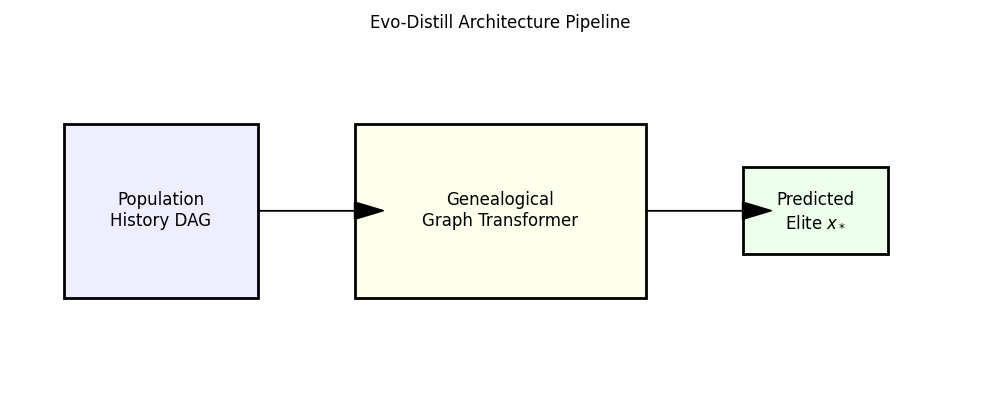
\includegraphics[width=0.95\linewidth]{figs/architecture.png}
    \caption{\textbf{Evo-Distill Architecture.} The framework treats evolutionary search as a genealogical graph process. \textbf{Left:} The input is a population history DAG, where nodes are individuals and edges represent mutation/crossover. \textbf{Middle:} A Graph-Causal Transformer uses masked attention to trace the ``lineage of success,'' learning which operators led to fitness gains. \textbf{Right:} references to the final elite are distilled into a ``one-shot'' prediction policy that bypasses iterative search at test time.}
    \label{fig:architecture}
\end{figure}
Conceptually, our work reframes evolutionary search as a source of demonstrations rather than solely a runtime algorithm. This opens several directions:
\begin{itemize}
    \item \textbf{Cross-domain priors.} EA trajectories collected in one domain (e.g., synthetic test functions) may transfer to related real-world problems via fine-tuning.
    \item \textbf{Theory of amortized search.} Understanding generalization properties of distilling from EAs, and characterizing when amortization is beneficial or harmful.
    \item \textbf{Integration with RL and design tools.} Using Evo-Distill as a front-end to RL, gradient-based methods, or human-in-the-loop design, providing fast candidate solutions that can be refined or inspected.
\end{itemize}

We see Evo-Distill as a step toward a broader goal: using powerful but expensive search procedures to train cheap, reusable models that internalize their heuristics and make global optimization more accessible across domains.

\nocite{*}
\bibliographystyle{plain}
\bibliography{refs}

\appendix

\section{Methodological Details}

\subsection{Genealogical Graph Construction}
We define the genealogical graph $G=(V, E)$ as follows:
\begin{enumerate}
    \item \textbf{Nodes}: Each node $v_{t,i}$ corresponds to individual $i$ in generation $t$.
    \item \textbf{Identity Edge}: If individual $i$ survives to generation $t+1$ (elitism), we add $v_{t,i} \to v_{t+1,i}$.
    \item \textbf{Mutation Edge}: If $v_{t+1,j}$ is a mutant of $v_{t,i}$, add $v_{t,i} \to v_{t+1,j}$ with edge attribute $a_{mut}$.
    \item \textbf{Crossover Edge}: If $v_{t+1,j}$ is cross-over from $v_{t,i}$ and $v_{t,k}$, add edges from both parents with attribute $a_{cross}$.
\end{enumerate}
The Graph Transformer uses strictly causal masking: $v_{t,i}$ can only attend to $\{v_{t', k} \mid t' < t\} \cup \{v_{t, k}\}$.

\subsection{Transformer Architecture}
We use a Graph-Causal implementation of GPT-2 small architecture:
\begin{itemize}
    \item \textbf{Layers}: 12
    \item \textbf{Hidden Dimension}: 768
    \item \textbf{Attention Heads}: 12
    \item \textbf{Context Window}: 1024 tokens (approx 10 generations of population size 100)
    \item \textbf{Population Encoder}: Set Transformer with 2 ISAB blocks.
\end{itemize}

\section{Experimental Setup}

\subsection{Data Generation}
We generate training data using a standard Genetic Algorithm (GA) teacher on the following distributions:
\begin{itemize}
    \item \textbf{Synthetic}: Shifted/Rotated Rastrigin, Ackley, Sphere ($D=50$).
    \item \textbf{Combinatorial}: traveling Salesman (TSP) on 20-50 nodes.
    \item \textbf{Control}: MuJoCo tasks (Hopper, Walker2d) optimizing linear policies learning policies (parameters $d \approx 200$).
\end{itemize}
We collect 100k trajectories for training, varying seed and instance parameters.

\subsection{Evaluation Metrics}
\begin{itemize}
    \item \textbf{Normalized Fitness}: $\frac{f - f_{min}}{f_{max} - f_{min}}$ relative to random search (0) and teacher convergence (1).
    \item \textbf{Speedup Factor}: $S = \frac{N_{EA}}{N_{student}}$, where $N$ is evaluations to reach 95\% teacher performance.
\end{itemize}

\end{document}
